\documentclass[12pt]{article}
\usepackage[utf8]{inputenc}
\usepackage{graphicx}
\usepackage{amsmath}
\usepackage{cite}
\title{
	{
\includegraphics[scale=0.3]{university.png}}\\
	{\large Amirkabir University of Technology}\\
	{A novel reinforcement learning algorithm for virtual network
		embedding}\\
	}
\author{Ali Zamani}
\date{30 June 2018}

\begin{document}


\maketitle

\newpage

\tableofcontents

\newpage

\section{Introduction}
 
Network Function Virtualization (NFV) aims to simplify service deployment using Virtual Network Functions (VNFs). Service deployment involves placement of VNFs and in-sequence routing of traffic flows through VNFs comprising a Service Chain (SC). The joint VNF placement and traffic routing is called SC mapping. In a Wide-Area Network (WAN), where several traffic flows, generated by many distributed node pairs, require the same SC; a single instance (or occurrence) of that SC might not be enough. SC mapping with multiple SC instances for same SC is a very complex problem, since sequential traversal of VNFs has to be maintained while accounting for traffic flows in various directions \cite{second}.

\subsection{Network Function Virtualization}
Traditionally, communication networks have deployed network services through proprietary hardware appliances (e.g., network functions such as firewalls, NAT, etc.) which are statically configured. With rapid evolution of applications, networks require agile and scalable service deployment.

Network Function Virtualization (NFV) \cite{first} offers a solution for an agile service deployment. NFV envisions traditional hardware functionality as software modules called Virtual Network Functions (VNFs). VNFs can be run on commercial-off-the-shelf hardware such as servers and switches in datacenters (DCs), making service deployment agile and scalable.
\subsection{Service Chain}
When several network functions are configured to provide a service, we have a “Service Chain”. The term “service chain” is used “to describe the deployment of such functions, and the network operator’s process of specifying an ordered list of service functions that should be applied to a deterministic set of traffic flows”. So, a “Service Chain” (SC) specifies a set of network functions configured in a specific order. With NFV, we can form SCs where VNFs are configured in a specific sequence that minimizes the bandwidth usage in the network \cite{third}. 

In Table \ref{table:1} we show some well-known Service Chains (SCs). \\
\begin{table}[t!]
\centering
\begin{tabular}{|c c|} 
 \hline
 Service Chains & Chained VNFs \\ [0.5ex] 
 \hline 
 Web Service & NAT-FW-TM-WOC-IDPS\\ 
VoIP &NAT-FW-TM-FW-NAT \\
 Video Streaming & NAT-FW-TM-VOC-IDPS \\
 Online Gaming&NAT-FW-VOC-WOC-IDPS\\[1ex] 
 \hline
\end{tabular}
\caption{Service Chain Requirements; Network Address Translator (NAT), Firewall (FW), Traffic Shaper (TM), WAN Optimization Controller (WOC), Intrusion Detection and Prevention System (IDPS), Video Optimization Controller (VOC).}
\label{table:1}
\end{table}

\subsection{Service Chain Mapping Issues}
Unfortunately, since VNFs in a single SC may need to be traversed by several distinct traffic flows (i.e., flows requested by multiple geographically-distributed node pairs) in a specific sequence, it becomes difficult to improve network resource utilization.

For example, consider Figure 1(a) and 1(b), where three traffic requests $r_1$ (from node 4 to 13), $r_2$ (from node 6 to 3), and $r_3$ (from node 14 to 1) demand SC $c_1$ composed of VNF1, VNF2, and VNF3 (to be traversed in this order VNF1$\rightarrow$ VNF2  $\rightarrow$ VNF3).

In Figure 1(a), if we consider only one mapping occurrence (or instance) for SC $c_1$, then some traffic flows (in our example, $r_3$ and $r_2$) will be ineffectively routed over long paths. Instead, as shown in Figure 1(b), if we use two SC instances for the same SC, we can improve network resource utilization, at the expense of a larger number of VNFs to be deployed (or replicated) in the network to serve the same SC. This results in a more complex problem when, in a Wide-Area Network (WAN), a large number of distributed node pairs generate traffic flows, creating heavy traffic demands. Our objective in this work is to reduce the network resource consumption for a WAN with heavy traffic demands.
%\begin{figure}[t!] \label{fig:1}
 % 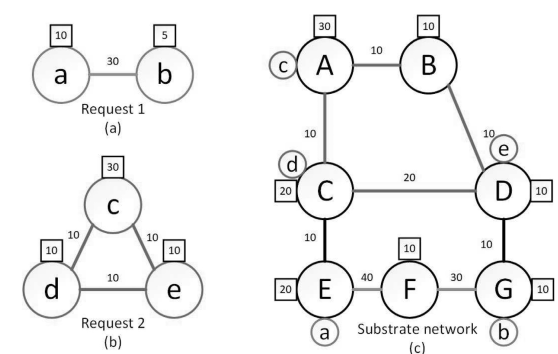
\includegraphics[width=\linewidth]{fig1.png}
  %\caption{Deploying more SC occurrence mappings reduces network resource consumption.}
%\end{figure}

So the question is: how many SC instances for the same SC are required for optimal network resource utilization?

A possible (trivial) solution to the problem of SC mapping in case of multiple node pairs requiring the same SC is to use one single instance that would most likely lead to host SCs at a single node (e.g., a DC) which is centrally located in the network. However, traffic flows may have to take long paths to reach the node hosting the SC, which will result in a high network resource consumption.

The other extreme case would be to use a distinct SC mapping per node pair (in other words, the number of SC instances is equal to the number of traffic node pairs). Now, we can achieve optimal network resource utilization as each node pair will use an SC effectively mapped along a shortest path in the network. However, this approach will increase the network orchestration overhead and increase capital expenditure, as there will be a large number of replicated VNF instances across nodes. To reduce excessive VNF replication, we bound the maximum number of nodes hosting VNFs.

Intuitively, the number of SC instances for a good solution will be a value between these two extremes. This solution will minimize the network resource utilization while not excessively increasing the number of nodes hosting VNFs \cite{Fourth}.
\subsection{Reinforcement algorithm}
The purpose of virtual network embedding is to map
virtual networks to a shared physical network while providing the
requests with adequate computing and bandwidth resources.
However, the virtual network embedding problem has been
proved to be NP-hard. As a result, a large number of heuris-
tic algorithms have been proposed, but most of them rely
on artificial rules to rank nodes or make mapping decisions.
parameters in these algorithms are always fixed and cannot be op-
timized, making the embedding decisions sub-optimally. On the
other hand, in prior works, the information about substrate net-
work and the knowledge about virtual network embedding hidden
in historical network request data have always been overlooked.

In recent years, big data, machine learning and artificial intel-
ligence have exciting breakthroughs achieving state of the art re-
sults such as natural language understanding and object detection.
Machine learning algorithms process a large amount of data col-
lected during a period and automatically learn the statistical in-
formation from the data to give classification or prediction.Rein-
forcement learning, as a widely-used technique in machine learn-
ing, has shown a great potential in dealing with complex tasks, e.g.,
game of go, or complicated control tasks such as auto-driving
and video games. The goal of a reinforcement learning system
(or an agent) is to learn better policies for sequential decision mak-
ing problems with an optimal cumulative future reward signal.

In this paper, we introduce reinforcement learning into the
problem of virtual network embedding to optimize the node map-
ping process. Similar to earlier works, our work is based on
the assumption that all network requests follow an invariable dis-
tribution. We divide our network request data into a training set and a testing set, to train our reinforcement learning agent (RLA)
and evaluate its performance respectively.We devise an artificial
neural network called policy network as the RLA, which observes
the status of substrate network and outputs node mapping results.
We train the policy network with historical network request data
using policy gradient through back propagation. An exploration
strategy is applied in the training stage to find better solutions, and
a greedy strategy is applied in evaluation to fully evaluate the ef-
fectiveness of the RLA. Extensive simulations show that the RLA is
able to extract knowledge from historical data and generalize it to
incoming requests.
\section{Network modeling}
In this section, we present a network model and formulate the
virtual network embedding problem with description of its com-
ponents. The notations used in this section are shown in table \ref{table:2}

\begin{table}[t!]
	\centering
	\begin{tabular}{|c l|} 
		\hline
		Notations & Descriptions \\ [0.5ex] 
		\hline 
		$G^s$ & Substrate network\\ 
		$N^s$ & Nodes of substrate network \\
		$L^s$ & Links of substrate network \\
		$A_N^s$& Node attribute of substrate network\\
		$A_L^s$&Link attribute of substrate network\\
		$G^v$& Virtual network of a certain virtual request\\
		$N^v$&Nodes of a virtual network\\
		$L^v$& Links of a virtual network\\
		$A^v_N$& Constraints of substrate nodes\\
		$A^v_L$& Constraints of substrate nodes\\
		\hline
	\end{tabular}
	\caption{Notations Descriptions}
	\label{table:2}
\end{table}
\begin{figure}[t!] \label{fig:1}
 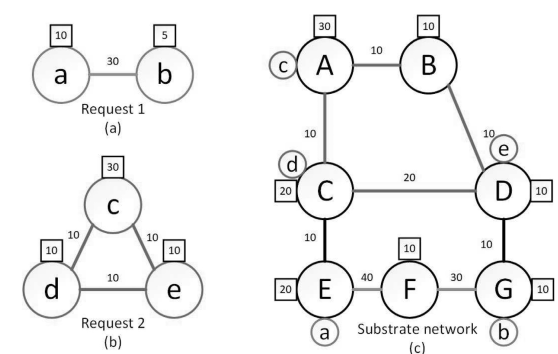
\includegraphics[width=\linewidth]{fig1.png}
\caption{An example of virtual network embedding.}
\end{figure}

Fig.\ref{fig:1} shows the mapping process of two different virtual net-
work requests. A substrate network is represented as an undi-
rected graph $G^s = (N^s, L^s, A_N^s, A_L^s)$ ,where $N^s$ denotes the set of all
the substrate nodes, $L^s$ denotes the set of all the substrate links,
$A^s_N$ and $A_L^s$ stand for the attributes of substrate nodes and links
respectively.

Fig.\ref{fig:1} (c)shows an example
of a substrate network, where a circle denotes a substrate node,
and a line connecting two circles denotes a substrate link. The
number in a square box denotes the CPU (computing) capacity of
that node, and the number next to a substrate link denotes the
bandwidth of that link. Similarly, we also use an undirected graph
$G^v = (N^v, L^v, A_N^v, A_L^v)$  to describe a virtual network request, where
$N^v$ denotes the set of all the virtual nodes in the request,$L^v$ de-
notes the set of all the virtual links in the request,$C_N^v$ and $C_L^v$ stand
for the constrains of virtual nodes and links respectively.

Fig. \ref{fig:1}(a) and (b) shows two different virtual re-
quests. Additionally, we use t to denote the arrival time of a virtual
request, and use t d to denote the duration of the virtual request.

When a virtual request arrives, the objective is to find a solu-
tion to allocate different kinds of resources in the substrate net-
work to the request while satisfying the requirements of the re-
quest. If such a solution exists, then the mapping process will be
executed, and the request will be accepted. Otherwise the request
will be rejected or delayed. The virtual network embedding pro-
cess can be formulated as a mapping M from $G^v$ to $G^s: G^v(N^v, L^v) \Rightarrow G^s(N^\prime, L^\prime)$

The main goal of virtual network embedding is to accept as
many requests as possible to achieve maximum revenue for an ISP,
when the arrival of virtual network requests follows an unknown
distribution of time and unknown resource requirements. Conse-
quently, the embedding algorithm must produce efficient mapping
decisions within an acceptable period.As shown in Fig.\ref{fig:1}, virtual
nodes a and b in request 1 are mapped to substrate nodes E and G
respectively, and virtual nodes c, d and e in request 2 are mapped
to substrate nodes A, C and D respectively. Note that the embed-
ding result of request 1 is not optimal. For example, the cost of
bandwidth in the substrate network can be significantly reduced
by moving a to F.
To determine the performance of embedding algorithms, most
works use certain metrics such as a long-term average revenue, a
long-term acceptance ratio, and a long-term revenue to cost ra-
tio. The revenue measures the profit of an ISP for accepting a cer-
tain virtual request, and it depends on the amount of requested
resources and the duration of it. Similar to the earlier works pre-
sented in, we define the revenue of accepting a virtual net-
work request as follows:
\begin{equation}
R(G^v, t, t_d) = t_d \times [\sum_{n^v \in N^v} CPU(n^v) + \sum_{l^v \in L^v} BW(l^v)]
\end{equation}

where CPU$(n^v)$ and BW$(l^v)$ denote the computing resource that
a virtual node $n^v$ requires and the bandwidth resource that a vir-
tual link $l^v$ requires respectively. Same as before, $N^v$ denotes the
set of all the virtual nodes in the request, and $L^v$ denotes the set
of all the virtual links in the request. As shown in the formula,
the revenue for accepting a virtual request is proportional to the
amount of requested resources and the duration of it.

When accepting a virtual request, the CPU consumption is al-
ways fixed, but the bandwidth consumption may vary depending
on the performance of embedding algorithm. Mapping a virtual
link to a shorter path in the substrate network will result in less
consumption of bandwidth resource. Therefore, a cost function is
formulated to measure the total amount of bandwidth resources
assigned to a virtual request, defined as follows:
\begin{equation}
C(G^v, t, t_d) = t_d \times [\sum_{l^v \in L^v} \sum_{l^s \in p^\prime_{l^v}} BW(l^v)]
\end{equation}

where $ p^\prime_{l^v}$ denotes the set of substrate links where virtual link $l^v$
is embedded. $C(G^v, t, t_d)$ computes the actual consumption of
bandwidth resource for embedding request $G^v$.
we use a long-term av-
erage revenue to evaluate the overall performance of our embed-
ding method defined as:

\begin{equation}
\lim\limits_{T \to \infty } \frac{\sum_{t= 0}^{T} R(G^v, t, t_d)}{T}
\end{equation}
where T is the time elapsed. A higher long-term average rev-
enue leads to a higher profit for the ISP. Another important metric
to evaluate the mapping algorithm is a long-term acceptance ratio,
which means the ratio of accepted requests to the total number
of requests arrived. A higher long-term acceptance ratio means the
proposed algorithm manages to serve more virtual requests.
Finally, a better utilization of substrate network resources
would lead to a high long-term average revenue with compara-
tively low cost of substrate network. The long-term revenue to cost
ratio, defined as follows, measures the utilization of substrate net-
work resources:
\begin{equation}
\lim\limits_{T \to \infty } \frac{\sum_{t= 0}^{T} R(G^v, t, t_d)}{\sum_{t= 0}^{T} C(G^v, t, t_d)}
\end{equation}


A higher long-term revenue to cost ratio shows that the pro-
posed algorithm is able to generate more profit with a compara-
tively less cost to network resources.
We will use these metrics mentioned above to evaluate the per-
formance of our embedding method in the following sections.

\section{Embedding algorithm}
In this section, we present the details of the proposed policy
network based reinforcement learning algorithm. Specifically, we
apply the reinforcement learning agent in the node mapping stage
to derive the probabilities of choosing nodes. The agent takes a
feature matrix extracted from the substrate network as input, and
makes decisions based on a policy network which is trained from
historical data.
\subsection{Feature extraction}
Every substrate node has several attributes, such as CPU ca-
pacity and the total amount of bandwidth of the adjacent links.
A thorough knowledge of substrate network is crucial for the re-
inforcement learning agent to establish a basic understanding of
its state and generate efficient mapping. To facilitate the agent to
choose the substrate nodes, we need to extract features of each
substrate node and use them as input to the policy network.

We extract four features for each substrate node listed as fol-
lows:
\begin{itemize}
	\item Computing capacity (CPU): The CPU capacity of a substrate
	node n S has a large impact on its availability. The substrate
	nodes with a higher computing capacity are likely to host more
	virtual nodes.
	\item Degree (DEG): The degree of a substrate node n S indicates the
	number of links connected to it. A substrate node with more
	adjacent links is more likely to find paths to other substrate
	nodes.
	\item Sum of bandwidth $(SUM^{(BW)})$: Every substrate node is con-
	nected to a set of links. A substrate node n S has a sum of band-
	width resources of its neighboring links:
	\begin{equation}
	SUM^{(BW)}(n^s) = \sum_{l^s \in L(n^s)}BW(l^s)
	\end{equation}
	where $L(n^s)$ is the neighboring links of $n^s$ and $BW(l^s)$ is the
	bandwidth resource of a substrate link $l^s$ . When a substrate
	node has access to more bandwidth, mapping a virtual node
	to it may lead to better link mapping options.
	\item  Average distance to other host nodes $AVG^{(DST)}$ : When mapping
	a virtual node, we also take into consideration the positions
	where other virtual nodes in the same request are mapped.
	By choosing a substrate node close to those already mapped,
	the cost of substrate link bandwidth can be reduced. We mea-
	sure the distance between two substrate nodes in terms of the
	number of links along the shortest path. The shortest path is
	computed following the FloydWarshall algorithm. We take
	an average of the distance from a substrate node $n^s$ to another host nodes $N^s$for the same request:
	\begin{equation}
	AVG^{DST}(n^s) = \frac{\sum_{n^s \in N^s}DST(n^s, n^s)}{|N^s| + 1}
	\end{equation}
	where $DST(n^s, n^s)$is the distance from node $n^s$ to node $n^s$.
\end{itemize}
In fact, the features that we can extract from the substrate
nodes would be far more than listed above. More features would
bring more information about the substrate network which leads
to a better performance of the learning agent. It should be noted
that extracting more features from the substrate network adds
complexity in computation.
After extracting the features of the kth substrate node $n_k^s$, we
take their normalized values and concatenate them into a feature
vector $v_k$ :

\begin{equation}
v_k = (CPU(n_k^s), DEG(n_k^s), SUM^{BW}(n_k^s), AVG^{DST}(n_k^s))^T
\end{equation}

The purpose of normalization is to accelerate the training pro-
cess and enable the agent to converge quickly. We concatenate all
feature vectors of substrate nodes to produce a feature matrix $M_f$
where each row is a feature vector of a certain substrate node:
\begin{equation}
M_f = (v_1, v_2, ..., v_{|N^s|})^T
\end{equation}

The feature matrix serves as an input to the learning agent. The
feature matrix is updated along with the changing substrate net-
work from time to time.

\subsection{Policy network}
Our work is based on the assumption that all network requests
follow an invariable distribution. As a result, if an embedding al-
gorithm works well for historical requests data, it is likely to have
the same performance for on-line virtual requests. In this work, we
implemented an artificial neural network called policy network as
the learning agent. It takes the feature matrix as input and out-
puts the probabilities of mapping virtual nodes to substrate nodes.
Then we train the policy network and optimize its performance on
historical virtual requests data in order to get comparative perfor-
mance for on-line virtual requests.

For simplicity, we build a simple policy network with basic ele-
ments of an artificial neural network as shown in Fig. \ref{fig:2} . The policy
network contains an input layer, a convolutional layer, a softmax
layer and finally a node filter. For each virtual node that requires
a mapping, we use the policy network to choose a substrate node
for it.
\begin{figure}[t!] \label{fig:2}
	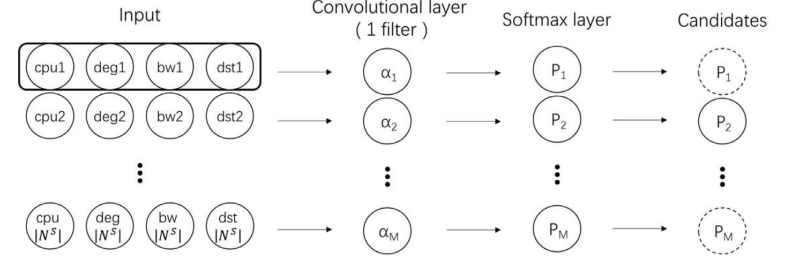
\includegraphics[width=\linewidth]{fig2}
	\caption{Policy network.}
\end{figure}

At the input layer, we compute the feature matrix and deliver
it to the policy network. The policy network then passes the in-
put feature matrix into a convolutional layer with one convolution
kernel, where the policy network evaluates the resources of each
substrate node. The convolutional layer performs a convolution op-
eration on the input to produce a vector representing the available
resources of each node:
\begin{equation}
h_k^c = w . v_k + b
\end{equation}

where $h_k^c$ is the kth output of the convolutional layer, $ω$ is the con-
volution kernel weight vector, and b is bias.

Then the vector is transmitted to a softmax layer to produce a
probability for each node which indicates the likelihood of yielding
a better result if mapping a virtual node to it. For the k th node, the
probability p k is computed as:

\begin{equation}
p_k = \frac{\exp(h_k^c)}{\sum_{i}\exp(h_k^c)}
\end{equation}

The softmax function is a generalization of the logistic regres-
sion. It turns the n-dimensional vector into real values between 0
and 1 that add up to 1. The output of the softmax function indi-
cates a probability distribution over n different possible mappings.
Some of the nodes are not able to host the virtual node in con-
cern because they do not have enough computing resources. We
add a filter to choose a set of candidate nodes with enough CPU
capacities.

\subsection{Training and testing}
We first randomly initialize the parameters in the policy net-
work, and train it for several epochs. For every virtual node in each
iteration, a feature matrix is extracted from the substrate network
which serve as input to the policy network. The policy network
outputs a set of available substrate nodes as well as a probability
for each node. The probability of each node represents the likeli-
hood that mapping a virtual node to it will yield a better result. In
the training stage, we cannot simply select the node with a max-
imal probability as the host because that the model is randomly initialized, which means the output could be biased and better so-
lutions might exist. In other words, we need to reach a balance
between the exploration of better solutions and the exploitation
of current model. To this end, we generate a sample from the set
of available substrate nodes according to their probability distri-
bution that the policy network outputs, and select a node as the
host. We repeat this process until all the virtual nodes in a virtual
request are assigned and proceed to link mapping. If no substrate
node is available, the mapping fails due to a lack of resources. For
link mapping, we apply a breadth-first search to find the shortest
paths between each pair of nodes.

In supervised learning, each piece of data in the training set
corresponds to a label indicating the desired output of the model.
With each output from model and the corresponding label, a loss
value is computed which measures the deviation between them.
The loss value for each piece of data in the training set sums up
to an aggregated loss value, and the training stage aims to mini-
mize the aggregated loss value. However, in reinforcement learn-
ing tasks such as virtual network embedding, data in the training
set does not have corresponding labels. The learning agent relies
on reward signals to know if it is working properly. A big reward
signal informs the learning agent that its current action is effective
and should be continued. A small reward signal or even a nega-
tive reward signal shows that the current action is erroneous and
should be adjusted. The choice of reward is critical in reinforce-
ment learning as it directly influences the training process and de-
termines the final policy. Here, we use the revenue to cost ratio of
a single virtual request as the reward for every virtual node in this
request because this metric represents the utilization efficiency of
the substrate resources. Then we apply policy gradient method to
train the policy network.
The actual implementation of the proposed algorithm is non-
trivial since we cannot provide each output with a label. As a re-
sult, we temporarily consider every decision that the agent makes
to be correct by introducing a hand-crafted label into our policy
network. Assume that we choose the i th node, then the hand-
crafted label in policy network would be a vector y filled with zeros
except the i th position which is one. Then we calculate the cross-
entropy loss:

\begin{equation}
L(y, p) = - \sum_{i}y_ilog(p_i)
\end{equation}

where $y_i$ and $p_i$ are the i th element of hand-crafted label and the
output of policy network respectively. We use backpropagation to
compute the gradients of parameters in the policy network. Since
we use hand-crafted label , we stack the gradients $g_f$ rather than
applying them immediately. If our algorithm fails to embed a vir-
tual request, the corresponding stacked gradients will be aborted
since we cannot determine the reward signal. If a virtual request
has been successfully mapped, we compute its revenue to cost ra-
tio as a reward r . Then we multiply the stacked gradients by using
the reward and an adjustable learning rate $\alpha$ to achieve the final gradients:

\begin{equation}
g = \alpha . r . g_f
\label{equ: 12}
\end{equation}


The learning rate $\alpha$ is introduced to control the magnitude of
gradients and the computation speed of training. If the gradients
are too large, the model becomes unstable and may not improve
through the training process. On the other hand, too small gra-
dients make training extremely slow. Therefore the learning rate
needs to be tuned carefully. It can be observed from Eq. \ref{equ: 12} larger
rewards make the corresponding gradients more significant than
small ones. As a result, the choices that lead to larger rewards
have larger impact on the learning agent, making it more prone
to make similar decisions. When we stack a batch of gradients, we
apply them to parameters and update the policy network. There
are two reasons for batch updating—one is that parameter updat-
ing normally takes a long time, but doing that in batches speeds up
this process. Another reason is that batch updating averages over
the gradients and is more stable. The training process is shown in
Algorithm \ref{alg: 1} . Lines 7–10 show node mapping stage where we com-
pute the gradients in line 10, lines 11–13 show the link mapping
stage.
In the testing stage, we apply a greedy strategy where we di-
rectly choose the node with the highest probability as the host.
The testing algorithm is shown in Algorithm \ref{alg: 2} .
\begin{figure}[t!] \label{alg:1}
	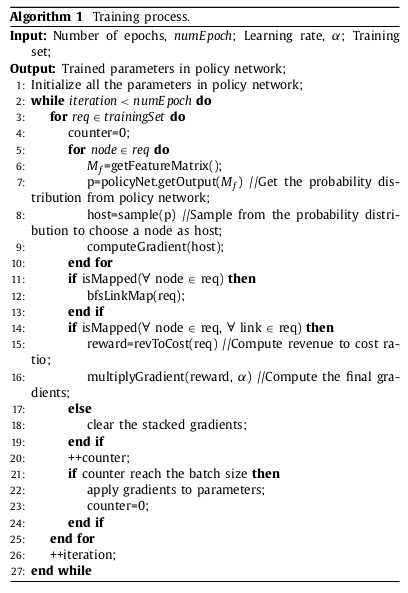
\includegraphics[width=\linewidth]{fig3}
	\caption{Training process.}
\end{figure}
\begin{figure}[t!] \label{alg:2}
	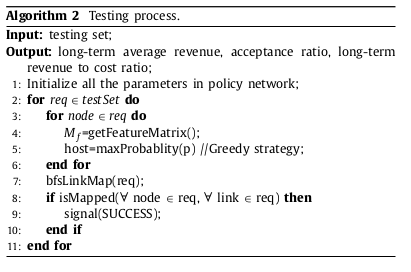
\includegraphics[width=\linewidth]{fig4}
	\caption{Testing process.}
\end{figure}

\section{Simulation}
\subsection{Simulation Parameters Declaration}
We tested our optimization process on a 14-node NSFNET WAN topology as shown in Figure \ref{network}. We generated 100 chains with up to 3 vnfs randomly. All of nodes can be NFV nodes. The link capacities are 100bps. Each traffic flow demand is up to 90 bps. Compute resource (CPU) at each NFV node is 100 cores per node. All other simulation parameters are shown in Table \ref{table:5}. All parameters can be change in Inputeconstants.py
\begin{figure}[t!]
\label{network}
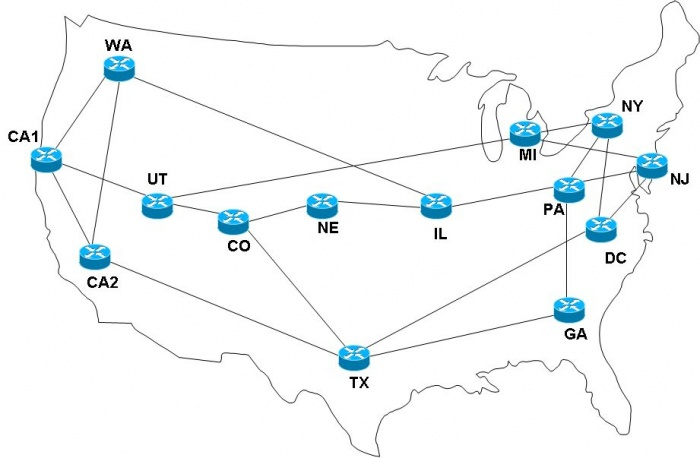
\includegraphics[scale=0.5]{nsfnet.jpg}
\caption{14-node NSFNET WAN topology.}
\end{figure}

\begin{table}[t!]
\centering
\begin{tabular}{|c c|} 
 \hline
 Parameter & Value \\ [0.5ex] 
 \hline 
 $G$ &It is shown in Figure \ref{network}\\ 
 $N^s$ & All nodes can be NFV node  \\
 $ epoch_num$ &  $Number of epochs: 100$ \\
 $batch_Size$ & $Number of batches: 4$ \\
 $node_features$& $Number of nodes' feature: 4$ \\
 $node_features$ & $1e-7$\\
 $chains_num$ & $Number of chains: 100$\\
 $fun_num$ & $ Number of functions in each chain: 3$\\
 $chain_ban$& $Maximum requiered bandwith of each chain: 90$ \\
 $cpu_range$& $Maximum requiered cpu core of each vertiual network: 3$\\
 $max_node_cap$& $Maximum cpu core of each node: 60$\\
 $min_node_cap$&$Minimum cpu core of each node: 30$\\
 $td_mean$& $Mean requiered time of each chain: 100$\\
 $td_std$& $Standard deviation of requiered time of each chain: 10$\\
 \hline
\end{tabular}
\caption{Simulation Parameters}
\label{table:5}
\end{table}
\subsubsection{Results}
Results of the simulation are shown in Fig. \ref{results}. In Fig. \ref{results}, loss and cost are decreasing and the reward is increasing but revenue is so wiggly. For future works, we can consider the source and destination for each chain and also extract more features for each node and use more complex policy network. 
\begin{figure}[t!]
	\label{results}
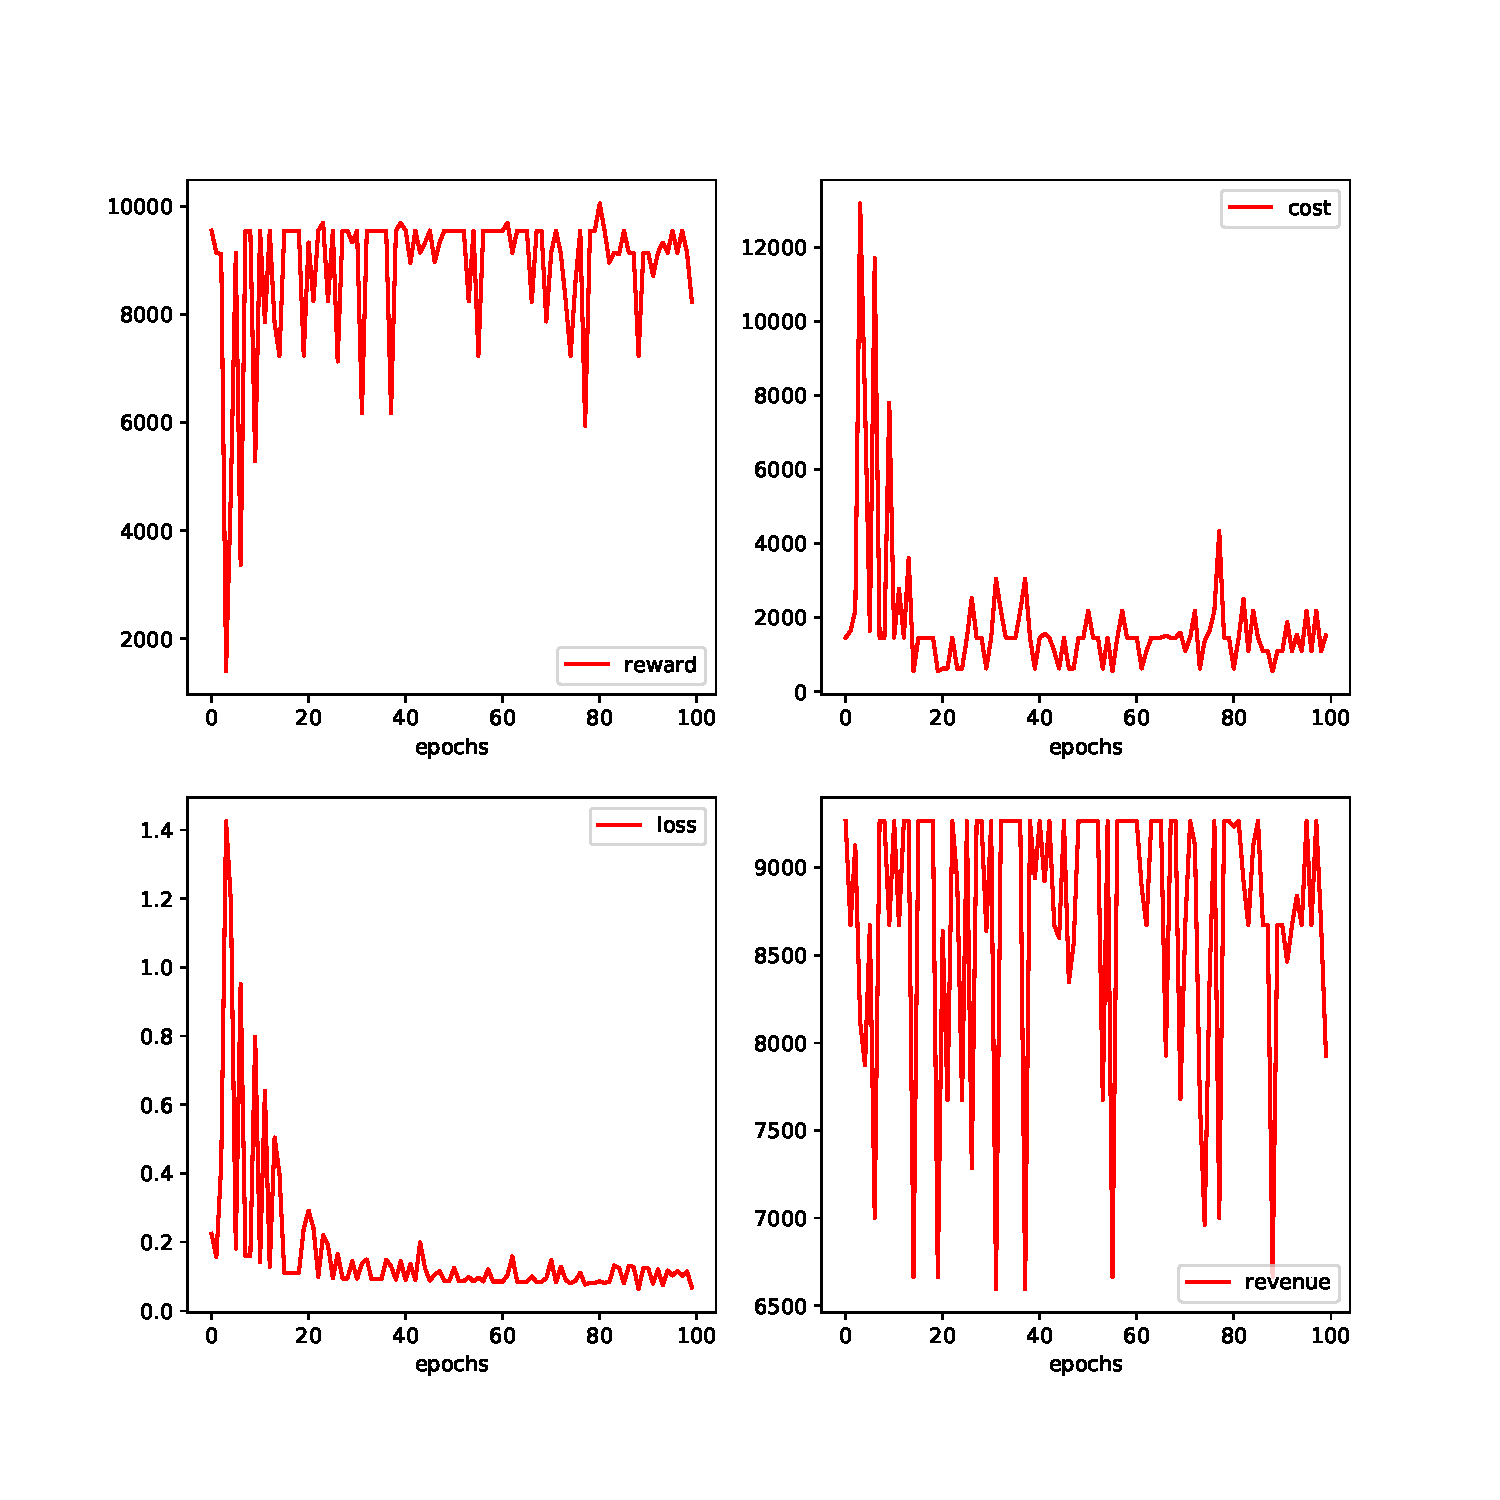
\includegraphics[scale=0.7]{results}
\caption{Results.}
\end{figure} 

\section{Conclusion}
I simulate this paper with TensorFlow and python is used. I also consider NFS-net network and 100 chains are generated randomly for training reinforcement learning algorithm. Eventually, I showed results. 
\clearpage

\addcontentsline{toc}{section}{References}
\bibliographystyle{IEEEtran}
\bibliography{IEEEabrv,ref}
\end{document}


